\documentclass[twoside]{article}

\usepackage{ustj}
\usepackage{tikz}
\usepackage{pgfplots}

\addbibresource{mss.bib}

\newcommand{\authorname}{Trent Steen}
\newcommand{\authorpatp}{\patp{hanfel-dovned}}
\newcommand{\affiliation}{Groundwire Foundation}

%  Make first page footer:
\fancypagestyle{firststyle}{%
\fancyhf{}% Clear header/footer
\fancyhead{}
\fancyfoot[L]{{\footnotesize
              %% We toggle between these:
              Manuscript submitted for review.\\
              % {\it Urbit Systems Technical Journal} I:1 (2024):  1–3. \\
              ~ \\
              Address author correspondence to \authorpatp.
              }}
}
%  Arrange subsequent pages:
\fancyhf{}
\fancyhead[LE]{{\urbitfont Urbit Systems Technical Journal}}
\fancyhead[RO]{Floating-Point Arithmetic on Deterministic Systems}
\fancyfoot[LE,RO]{\thepage}

%%MANUSCRIPT
\title{Groundwire Comet Cryptography}
\author{\authorname~\authorpatp \\ \affiliation}
\date{}

\begin{document}

\maketitle
\thispagestyle{firststyle}

\begin{abstract}
\emph{Adapted from \textsc{uip}-XXX.}
\end{abstract}

% We will adjust page numbering in final editing.
\pagenumbering{arabic}
\setcounter{page}{1}

\tableofcontents

\section{Introduction}

Groundwire allows comets to rotate their networking keys. How does this
work precisely?

\section{Elliptic Curves}\label{elliptic-curves}

\begin{quote}
``Each Urbit ship possesses two networking keypairs: one for encryption, and one for authentication. We often refer to these two keypairs as though they were a single keypair because they are stored as a single atom. Elliptic Curve Diffie-Hellman is used for encryption, while Elliptic Curve Digital Signature Algorithm is used for authentication.''  (\href{https://docs.urbit.org/urbit-os/kernel/ames/cryptography#key-exchange}{Urbit docs, ``Ames Cryptography''})
\end{quote}

An \emph{elliptic curve} is a two-dimensional curve defined by the
general form $y^{2} = x^{3} + ax + b$ with the special
condition that $4a^{3} + 27b^{2} \neq 0$. As long as that
special condition holds true for whatever constants you picked for $a$ and $b$, you can define a special type of addition for pairs of points on this curve where you draw a line between them, find the singular third point on the curve that this line hits, $c$, and then flip that third point across the $x$ axis, $-c$ (see Figure~\ref{fig:elliptic-curve}). Multiplication means doing this process repeatedly.

\begin{figure}[h]
  \centering
  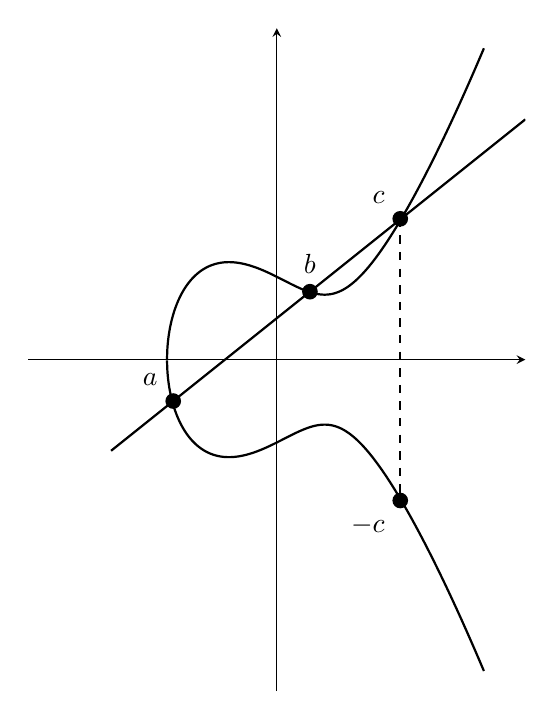
\begin{tikzpicture}
    \begin{axis}[
      axis lines=center,
      xlabel={},
      ylabel={},
      xmin=-3, xmax=3,
      ymin=-4, ymax=4,
      samples=100,
      smooth,
      width=10cm,
      height=10cm,
      axis equal image,
      ticks=none
    ]
    
    % Draw the elliptic curve: y^2 = x^3 - x + 1
    \addplot[
      domain=-2:2.5,
      thick,
      black,
      samples=2000
    ] ({x}, {sqrt(x^3 - x + 1)});
    
    \addplot[
      domain=-2:2.5,
      thick,
      black,
      samples=2000
    ] ({x}, {-sqrt(x^3 - x + 1)});

    % Draw the line through P, Q, and R
    \addplot[
      domain=-2:3,
      thick,
      black
    ] {0.8*x + 0.5};
    
    % Mark and label the points
    \node[circle, fill=black, inner sep=2pt, label=above left:$a$] at (axis cs:-1.25,-0.5) {};
    \node[circle, fill=black, inner sep=2pt, label=above:$b$] at (axis cs:0.4,0.82) {};
    \node[circle, fill=black, inner sep=2pt, label=above left:$c$] at (axis cs:1.49,1.70) {};
    \node[circle, fill=black, inner sep=2pt, label=below left:$-c$] at (axis cs:1.49,-1.70) {};
    \draw[dashed, thick, black] (axis cs:1.49,1.70) -- (axis cs:1.49,-1.70);
    
    \end{axis}
  \end{tikzpicture}
  \caption{Elliptic curve point addition and multiplication, with the curve $y^2 = x^3 - x + 1$.}
  \label{fig:elliptic-curve}
\end{figure}

Why would you do such a thing? Because it's irreversible. A private key is just a number; a public key is just that number multiplied by some other commonly agreed on number (the ``base point'') using elliptic curve arithmetic. Regular multiplication would mean that you could trivially obtain someone's private key by dividing their public key by the base point, but by bouncing all our operations around with elliptic curve multiplication, we prevent division.  This is less crude and more beautiful than it might seem, because these keypairs have some special properties that are useful for cryptography.

If I multiply my private key by your public key, I get the same answer as if you multiply your private key by my public key. This allows us to use that answer as a shared secret that only the two of us know. In the \emph{Elliptic Curve Diffie-Hellman (\textsc{ecdh})} protocol, we take the $x$ coordinate of that shared secret and run it through a key derivation function (in Urbit's case, \textsc{sha}-256) to get a symmetric key which allows us to both encrypt and decrypt messages. Using this key, we can communicate privately.

Similarly, \emph{Elliptic Curve Digital Signature Algorithm (\textsc{ecdsa})} uses a more extensive algorithm to allow me to sign a message with my private key and for you to use my public key to verify that I did in fact sign it.

The elliptic curve that Urbit uses for key generation is the fast and
un-patented \emph{Curve25519}. This specifies the curve equation, the base point, and the finite field (the range of integers that we operate on, wrapping back to 0 if we go over the max value). There are two algebraically equivalent representations of Curve25519 that Urbit uses, with each defining its own set of standard operations: Montgomery Form (X25519), which is more efficient for \textsc{ecdh}, and Twisted Edwards Form (Ed25519), which is more efficient for \textsc{eddsa} (an elliptic curve signature scheme so similar to \textsc{ecdsa} that Urbit's docs at one point confused the two).

Urbit implements the Ed25519 standard operations in its
\lstinline[style=inlinecode]{+ed:crypto} zuse core for \textsc{eddsa}, along with a few X25519-like
operations for \textsc{ecdh}. My co-author Chat\textsc{gpt} can elaborate:

\begin{quote}
\sloppy
scam: scalar multiply. Takes a point and a scalar → returns scalar ×
point. This is the core elliptic curve operation. ward: point addition
(Edwards curve formula). Needed for scalar multiplication by repeated
doubling-and-adding. etch / deco: encode/decode a curve point into/from
an atom. This is how keys are serialized. luck: derive a keypair (public
+ private) from a seed. This is how comets/\-planets get Curve25519 keys.
puck: get the public key from a seed. slar / shar: perform a
Diffie--Hellman secret derivation (\textsc{ecdh}). Given your private scalar and
someone else's public point, return a shared secret. sign / sign-raw /
sign-octs: produce signatures. This is the \textsc{ecdsa}/\textsc{eddsa}-like
functionality. veri / veri-octs: verify signatures against a public key.
\end{quote}

With all of this context, you can imagine why we'd want to have two
pairs of networking keys: \textsc{ecdh} encryption and \textsc{eddsa} signatures are both complicated mathematical operations, so it's cleaner and safer to delineate between the two protocols completely in case of implementation bugs, future cryptographic discoveries, nonce reuse, and key rotations.

So how are these keypairs turned into an atom, where are they stored,
and when are they used?

\section{Asymmetric Cryptosuites}\label{asymmetric-cryptosuites}

The usage of public and private keys we've described so far is called
\emph{asymmetric cryptography}. Ames defines its own standard interface for asymmetric cryptography in the \lstinline[style=inlinecode]{+acru} core: \newpage

\begin{lstlisting}[style=listingcode]
++  acru
  ::  opaque object
  $_  ^?
  |%
  ::  asymmetric ops
  ++  as  ^?
    |%
    ::  encrypt to a
    ++  seal  |~([a=pass b=@] *@)
    ::  certify as us
    ++  sign  |~(a=@ *@)
    ::  authenticate from us
    ++  sure  |~(a=@ *(unit @))
    ::  accept from a
    ++  tear  |~([a=pass b=@] *(unit @))
    --  ::as
  ::  symmetric de, soft
  ++  de  |~([a=@ b=@] *(unit @))
  ::  symmetric de, hard
  ++  dy  |~([a=@ b=@] *@)
  ::  symmetric en
  ++  en  |~([a=@ b=@] *@)
  ::  export
  ++  ex  ^?
    |%
    ++  fig  *@uvH            ::  fingerprint
    ++  pac  *@uvG            ::  default passcode
    ++  pub  *pass            ::  public key
    ++  sec  *ring            ::  private key
    --  ::ex
  ::  reconstructors
  ++  nu  ^?
    |%
    ::  from [width seed]
    ++  pit  |~([a=@ b=@] ^?(..nu))
    ::  from ring
    ++  nol  |~(a=ring ^?(..nu))
    ::  from pass
    ++  com  |~(a=pass ^?(..nu))
    --  ::nu
  --  ::acru
\end{lstlisting}

\noindent
Note the \lstinline[style=inlinecode]{^?} ketwut runes: this is a lead core, an interface. Ames expects to be provided with an implementation of these functions that can slot in here. In current Arvo, the only existing implementation is \lstinline[style=inlinecode]{+crub:crypto} in zuse:

\begin{quote}
seal: encrypt to a peer. Runs \textsc{ecdh} with our enc secret + their enc
pubkey, hashes with \textsc{sha}-256, signs with our auth secret, encrypts with
\textsc{aes}-\textsc{siv}. sign: sign a message with our auth secret (\textsc{eddsa}). sure: verify
a message was signed with the matching auth pubkey. tear: decrypt from a
peer. \textsc{ecdh} with our enc secret + their enc pubkey, \textsc{sha}-256, \textsc{aes}-\textsc{siv}
decrypt, then verify signature.

fig: \textsc{sha}-256 fingerprint of the public key(s). pac: \textsc{sha}-256 fingerprint
of the secret key(s). pub: concatenate enc pubkey + auth pubkey into one
atom. sec: concatenate enc secret + auth secret into one atom.

pit: generate a new keypair from a seed. Uses \textsc{sha}-512 for privates,
\lstinline[style=inlinecode]{+puck:ed:crypto} for publics. nol: reconstruct a \lstinline[style=inlinecode]{+crub} from a
secret key atom. com: reconstruct a \lstinline[style=inlinecode]{+crub} from a public key atom.
\end{quote}

Here we have the key derivation and signing functions as wrappers around \lstinline[style=inlinecode]{+ed:crypto} and \lstinline[style=inlinecode]{+aes:crypto}, along with arms for turning networking keys into atoms and atoms back into \ldots{} \lstinline[style=inlinecode]{+crub}s? You'd think that we'd turn an atom back into a pair of networking keys. Right?

But what if you wanted to use a different cryptosuite with Ames? Then all of your old keys would be stranded as incompatible atoms. By using a \lstinline[style=inlinecode]{+crub} object instead, with keys in its payload and a battery for how to use them, we maintain consistency even if there were multiple implementations of \lstinline[style=inlinecode]{+acru}.

We do, then, need to track which cryptosuite to decode a key atom
to---so we store this in the Jael secrets vane right next to the keys themselves:

\begin{lstlisting}[style=listingcode]
+$  point
  $:  =rift
      =life
      keys=(map life [crypto-suite=@ud =pass])
      sponsor=(unit @p)
  ==
\end{lstlisting}

Now we can begin to home in on exactly what needs to change in the Urbit crypto suite in order for Groundwire to allow comets to rotate their keys.

In current Arvo, when a comet contacts another ship, that ship will ask the comet for an \emph{unecrypted self-attestation packet} to prove that the sender does in fact control the private key whose public counterpart was hashed into the comet's \lstinline[style=inlinecode]{@p}:

\begin{lstlisting}[style=listingcode]
::  +request-attestation: helper to request
::  attestation from comet. Also sets a timer
::  to resend the request every 30s.
::
++  request-attestation
  |=  =ship
  ^+  event-core
  =+  (ev-trace msg.veb ship |.("requesting attestion"))
  =.  event-core
    =/  =blob  (sendkeys-packet ship)
    (send-blob for=| ship blob (~(get by peers.ames-state) ship))
  =/  =wire  /alien/(scot %p ship)
  (emit duct %pass wire %b %wait (add now ~s30))
\end{lstlisting}

But Groundwire comets don't self-attest to their identity; that
attestation comes into Jael via \lstinline[style=inlinecode]{%ord-watcher} in the same way that
Azimuth attestations come into Jael via \lstinline[style=inlinecode]{%azimuth} and \lstinline[style=inlinecode]{%eth-watcher}. In the Groundwire codebase, the \lstinline[style=inlinecode]{+request-} \lstinline[style=inlinecode]{attestation} arm is
replaced with:

\begin{lstlisting}[style=listingcode]
++  fetch-comet-pki
  |=  =ship
  ^+  event-core
  =+  (ev-trace msg.veb ship |.("requesting attestion"))
  =/  lyf
    (rof [~ ~] /ames %j `beam`[[our %lyfe %da now] /(scot %p ship)])
  ?:  ?=([~ ~ [* * ^]] lyf)
    =.  event-core  (emil moves)
    (emit [[//keys]~ %pass /public-keys %j %public-keys ship ~ ~])
  =.  event-core
    =/  =blob  (sendkeys-packet ship)
    (send-blob for=| ship blob (~(get by peers.ames-state) ship))
  =/  =wire  /alien/(scot %p ship)
  (emit duct %pass wire %b %wait (add now ~s30))
\end{lstlisting}

If we have this comet's networking keys in Jael (and thus lyf is not
null), then instead of asking the comet to self-attest, we check our
recorded networking keys. So far, so good: even though we're still
expecting the comet's \lstinline[style=inlinecode]{@p} to match its public key in the non-Groundwire wutcol branch, we can skip that check and trust Jael for Groundwire
comets. So why do we need to change our crypto suite?

\section{Tweaked Keys}\label{tweaked-keys}

\emph{{[}Note: this section is slightly out of date, because we use
\lstinline[style=inlinecode]{+cric} now, which includes a second field to store tweak data
in.{]}}

Groundwire's proposed change to comet attestation has greater
philosophical implications for identity than you might expect.

Groundwire's strategy is to bet on Bitcoin being the one true long-term
substrate that Urbit's \textsc{pki} will live on, because Bitcoin is the only
chain that offers an unambiguous protocol-level definition of canonical
history (``the longest valid proof-of-work chain'') that a Kelvin 0
Urbit could resolve without appeal to social coordination or trusted
checkpoints.

But it \emph{is} a bet, and a contentious one at that in an ecosystem
that includes Ethereum and Nockchain. For this reason, we \emph{don't}
insist that Jael only ingest comet \textsc{pki} data from Bitcoin.

All of Groundwire's changes to Arvo stem from modifying Ames's
\lstinline[style=inlinecode]{+request-attestation} arm to \lstinline[style=inlinecode]{+fetch-comet-pki}, with the
core proposition being that comets have the ability to publish their
networking keys to any source of \textsc{pki} truth that other Urbit ships choose
to interpret. To enable this, comets need to somehow encode within Jael
\emph{which} \textsc{pki} they've attested to. This is where tweaked keys come
in.

The payload of \lstinline[style=inlinecode]{+crub} is:

\begin{lstlisting}[style=listingblock]
[pub=[cry=@ sgn=@]\ sek=(unit [cry=@ sgn=@])]
\end{lstlisting}

An encryption public key, a signing public key, and optionally their
secret counterparts.

The Groundwire codebase introduces a new \lstinline[style=inlinecode]{+acru}-compatible
crypto-suite, \lstinline[style=inlinecode]{+cryc}, with the payload:
\begin{lstlisting}[style=listingblock]
$%  $:  suite=%b
        pub=[cry=@ sgn=@ ~]
        sek=$@(~ [sed=@ cry=@ sgn=@])
    ==
    $:  suite=%c
        pub=[cry=@ sgn=@ tw=[ugn=@ dat=@]]
        sek=$@(~ [sed=@ cry=@ sgn=@])
==  ==
\end{lstlisting}

\noindent
We refer to \lstinline[style=inlinecode]{+crub} as ``Suite B'' because it implements the \textsc{nsa} Suite B Cryptography Standard. \lstinline[style=inlinecode]{+cryc} includes everything in Suite B, along with a new ``Suite C'' (a coinage of our own).

The Suite C payload's main difference is that the signing keys are ``tweaked.'' We store \lstinline[style=inlinecode]{ugn}, the untweaked public key, and \lstinline[style=inlinecode]{sed}, the random seed used to originally generate our untweaked keypair, so that we have everything we need to recreate them if we ever need to. Then, we can tweak them by passing them into a tweaking function along with a bytestring, \lstinline[style=inlinecode]{dat}:

\begin{lstlisting}[style=listingblock]
::  pub.s = public signing key
::  sek.s = private signing key
=/  mit  (shax (can 3 [32 pub.s] [(met 3 dat) dat] ~))
(scad:ed pub.s sek.s mit)
\end{lstlisting}

First, the public key is hashed along with the data to produce \lstinline[style=inlinecode]{mit}, the ``tweak scalar.'' All three of these arguments get passed into \lstinline[style=inlinecode]{+scad:ed}, a wrapper around two other \lstinline[style=inlinecode]{+ed} arms:

\begin{lstlisting}[style=listingblock]
::  scalar addition on public and private keys
++  scad
  ~/  %scad
  |=  [pub=@uxpoint sek=@uxscalar sca=@uxscalar]
  ^-  [pub=@uxpoint sek=@uxscalar]
  [(scap pub sca) (scas sek sca)]
\end{lstlisting}

\noindent
And these two arms, \lstinline[style=inlinecode]{+scap} and \lstinline[style=inlinecode]{+scas}, simply perform elliptic curve addition between the tweak scalar and the corresponding key!

Anyone with both your public untweaked key and your tweak data can
recreate your tweaked key. And, sure enough, we recall the
\lstinline[style=inlinecode]{$point:jael} type:

\begin{lstlisting}[style=listingblock]
+$  point
  $:  =rift
      =life
      keys=(map life [crypto-suite=@ud =pass])
      sponsor=(unit @p)
  ==
\end{lstlisting}

\noindent
wherein the \lstinline[style=inlinecode]{$pass} field is the atom that, in Suite B, encodes the two public keys. In Suite C, it encodes the encryption key, the untweaked signing key, \emph{and} the tweak data. Upon receiving a message from a comet, your ship can reconstruct the tweaked key and check if it matches the key that the comet provides.

This might seem like a ton of unnecessary work. If you already trust Jael's sources of truth (\lstinline[style=inlinecode]{%ord-watcher}, in this case), why bother with tweaked keys at all?

The reason is that, if we have potentially arbitrary sources of \textsc{pki} truth, then we need an extra degree of freedom to point back to it. The tweak provides that pointer by baking it directly into the networking key itself, ensuring that the two can never drift apart (whether through a replay attack or an indexing bug).

In Groundwire's implementation, that anchor is the ordinal number of the sat used for the comet's inscription. When \lstinline[style=inlinecode]{%ord-watcher} sees an attempted key rotation, it checks the specified comet ID's \lstinline[style=inlinecode]{$pass} in Jael to verify that the transaction's ordinal number matches the current tweak data, and rejects it if it doesn't. Back in userspace, any agent can later recompute the tweak to confirm that the key they're communicating with really does originate from the expected on-chain inscription.

This tweaked key protocol enables a new conception of identity on Urbit: rift, life, keys, \emph{and data}. The additional field here could be used for a lot more than just ordinals!

\section{Routing}\label{routing}

The final implication of Groundwire's change to Ames' interpretation of comet provenance is that, since Groundwire comets articulate a network independent of Azimuth, they shouldn't need to rely on the current sponsorship hierarchy for packet routing. To facilitate this, comets can include include another piece of info in their attestations, called a \lstinline[style=inlinecode]{$fief}:

\begin{lstlisting}[style=listingblock]
+$  fief
  $%  [%turf p=(list turf) q=@udE]
      [%if p=@ifF q=@udE]
      [%is p=@isH q=@udE]
  ==
\end{lstlisting}

\noindent
\lstinline[style=inlinecode]{$point:jael} is updated to contain a \lstinline[style=inlinecode]{(unit\ fief)}, potentially storing the comet's static IP address (\lstinline[style=inlinecode]{%if} for \textsc{ipv}4 or \lstinline[style=inlinecode]{%is} for \textsc{ipv}6) or domain (\lstinline[style=inlinecode]{%turf}).

On top of this, Ames has been updated to allow any ship to be a valid
sponsor, necessitating a few changes to its routing logic to detect
cycles and ensure that sponsorship chains are allowed to terminate in
any sponsor with a \lstinline[style=inlinecode]{$fief}, rather than only in galaxies.

\subsection{Sources}\label{sources}

\begin{quote}
https://en.wikipedia.org/wiki/Curve25519
https://docs.urbit.org/urbit-os/kernel/arvo/cryptography
\url{https://docs.urbit.org/urbit-os/kernel/ames/cryptography\#comets\#}
https://docs.urbit.org/hoon/cryptography\#ed
https://www.youtube.com/watch?v=NF1pwjL9-DE
https://docs.google.com/document/d/1GbrxMvFeL51\_Q0ieXyXeN21ylrlBkOzeF1eo9iw5Yak/edit?tab=t.nzlzmcdsxd5\#heading=h.jmr099yfrej5
https://github.com/orgs/gwbtc/discussions/12
\end{quote}

\emph{I didn't do a very good job of tagging specific citations in this
write-up, so keep in mind if this ever gets adapted for public
consumption that I probably stole \textasciitilde tinnus's phrasing in a
couple places, and certainly wrote this on the back of his work.}
\tombstone

\selectlanguage{USenglish}
% \printbibliography
\end{document}
